\begin{figure*}[t]
\centering
\subfigure[]{
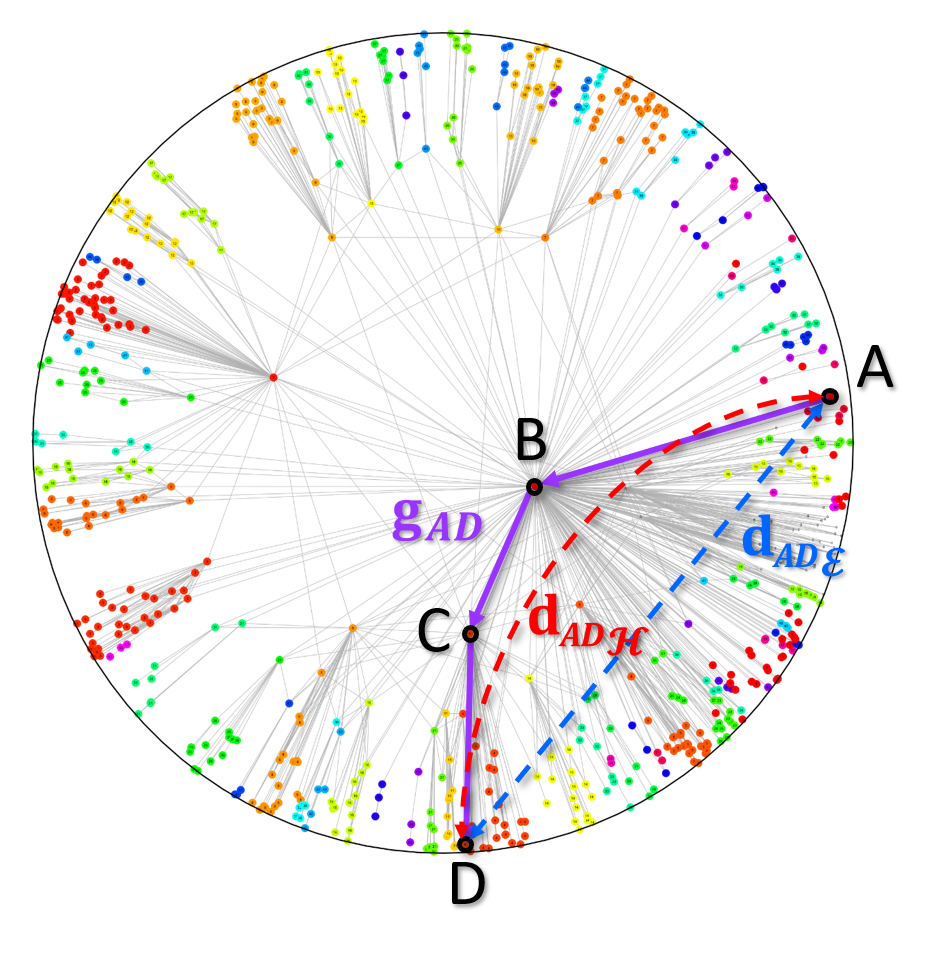
\includegraphics[width=0.24\linewidth]{figure/fig1_a.png}
\label{example:a}
%\caption{fig1}
}%
\subfigure[]{
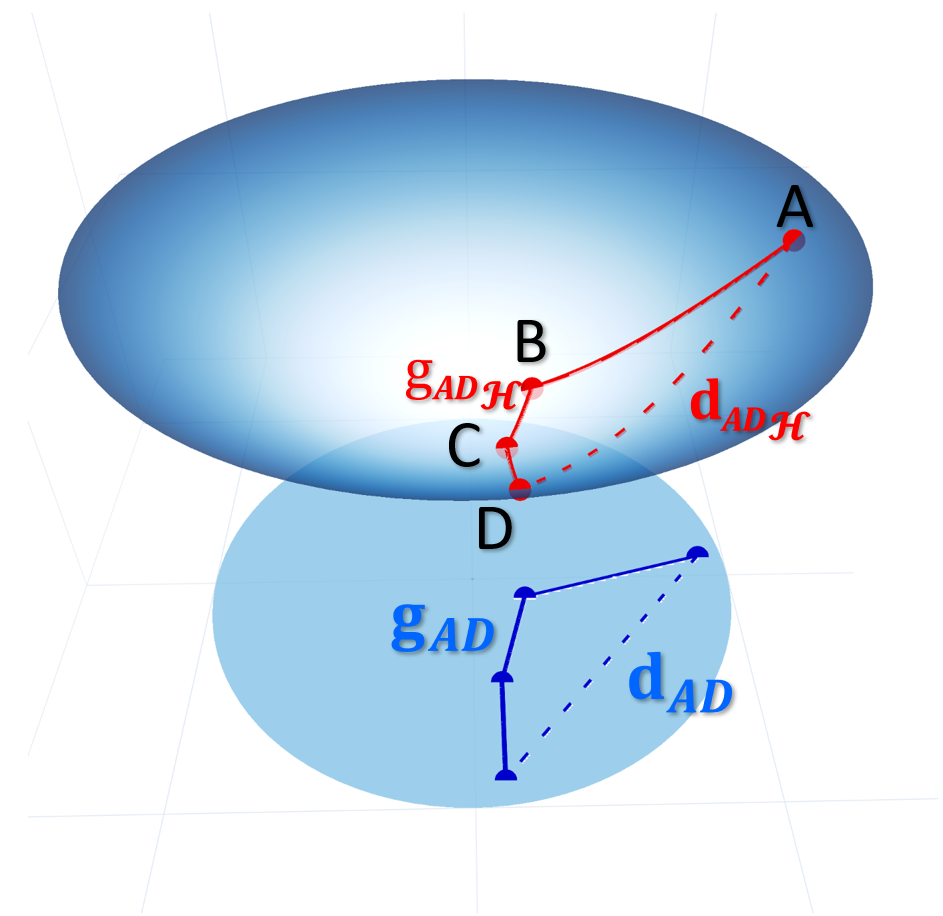
\includegraphics[width=0.24\linewidth]{figure/fig1_b.png}
\label{example:b}
%\caption{fig2}
}%
\subfigure[]{
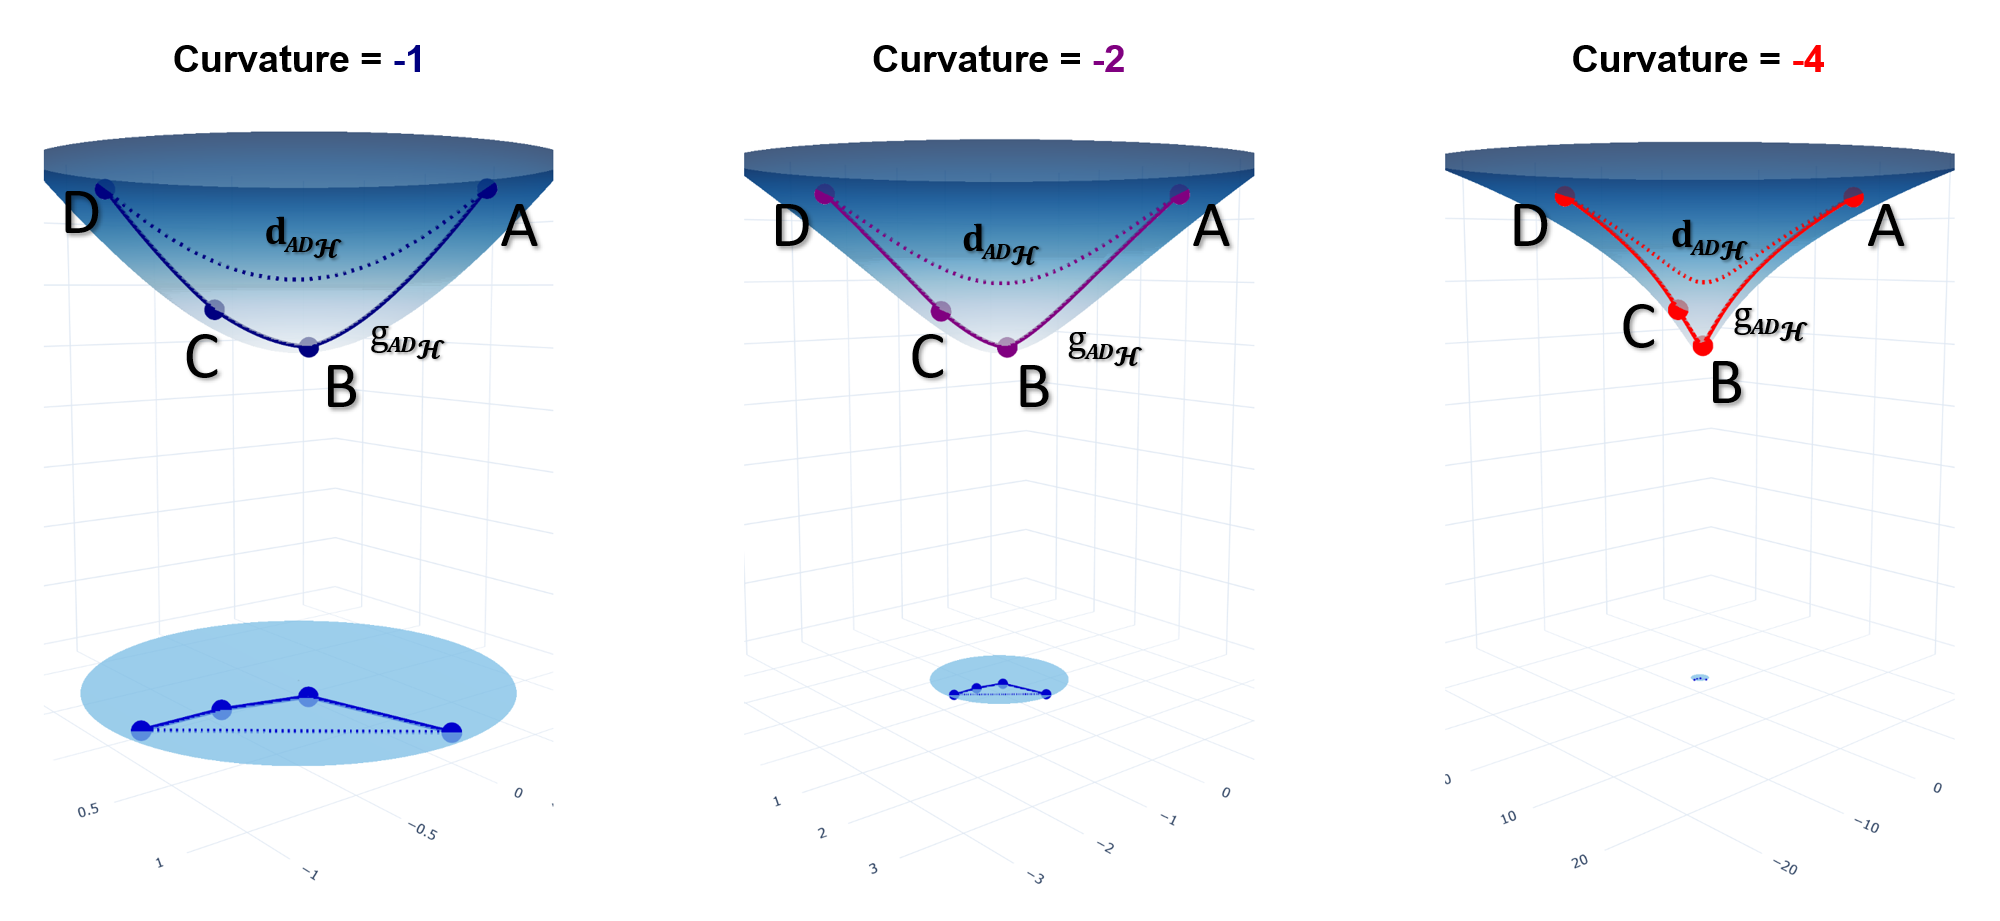
\includegraphics[width=0.52\linewidth]{figure/fig1_c.png}
\label{example:c}
}
\centering
\caption{An illustration of different distance metrics in hyperbolic spaces with different curvature. 
(a) Graph distance (\textcolor{purple}{purple solid lines}), Euclidean distance (\textcolor{blue}{blue dashed}) and hyperbolic geodesics(\textcolor{red}{red dashed curve}) on a tree-like graph in Poincaré disk; 
(b) Graph distance and embedded distance in Poincaré disk (Euclidean projection, \textcolor{blue}{blue solid and dashed lines}) and hyperboloid (Curvature $K = -1$ \textcolor{red}{red solid and dashed curves}); 
(c) Graph distance and hyperbolic distance on the hyperboloid of different curvature. }
\label{example}
\end{figure*}

\section{Curvature versus Hierarchical Structure}
\label{section 3}
In this section, we perform a qualitative analysis to reveal the intrinsic connections between curvature and the hierarchical structure. 
We illustrate a hyperbolic space tree-like graph as an example on Poincaré disk as shown in Figure~\ref{example:a}. 
To help explain our observation, we define two important distances as follows: 

%Distance introduction%
\textbf{Graph distance. }
Graph distance represents the length of the shortest path between two nodes on a graph.
Propagating information is an essential function of many real networks (e.g., Internet, brain, regulatory, metabolic networks). 
We can use information propagation to measure the topological distance between two nodes in graph representation learning. 
The graph distance $\mathbf{g_{i j}}$ between node $i$ and node $j$ is defined as follows: 
\begin{equation}\label{graphdist}
    \mathbf{g}_{i j} = \mathbf{d}_{i k_1} + \mathbf{d}_{k_1 k_2} + \mathbf{d}_{k_2 k_3} + \cdots + \mathbf{d}_{k_n j},
\end{equation}
where $k_1,k_2,\cdots,k_n$ are the nodes on the shortest path between node $i$ and node $j$, and $\mathbf{d}$ is the embedded distance between two nodes. 
In the Figure~\ref{example:a}, the graph distance between nodes $A$ and $D$ (\textcolor{purple}{purple solid lines}) is $\mathbf{g}_{AD}=r_{AB}+r_{BC}+r_{CD}$. 

\textbf{Embedded distance. }
Embedded distance represents the distance between two nodes in the embedded space (dashed lines in Figure~\ref{example}), which can be regarded as the semantic distance or feature similarity between two nodes in machine learning. 
We use $\mathbf{d}_{\mathcal{E}}$ and $\mathbf{d}_{\mathcal{H}}$ to denote the embedding distance in Euclidean and hyperbolic embedding spaces, which can be computed by the inner product and the Lorentzian scalar product, respectively. 
The example is shown in Figure~\ref{example:a}. 
For the nodes $A$ and $D$, their Euclidean embedded distance is $\mathbf{d}_{^{AD}\mathcal{E}}$ (\textcolor{blue}{blue dash line}), and the hyperbolic distance is $\mathbf{d}_{^{AD}\mathcal{H}}$ (\textcolor{red}{red dash curve}). 

%Distance computation%
Now, we show how hyperbolic distance changes with curvature as follows. 
Here, we employ the following conclusions from the existing work of hyperbolic geometry in complex network~\cite{Krioukov2010Hyperbolic} to analyze the hyperbolic distance metrics: 
The hyperbolic space of constant curvature is defined as $K = -{\zeta}^2 < 0, \zeta > 0$. 
The hyperbolic distance $\mathbf{d}_{\mathcal{H}}$ between two nodes at polar coordinates $(r, \theta)$ and $(r^{\prime}, \theta^{\prime})$ is given by the hyperbolic law of cosines:
\begin{equation}\label{hyperdist1}
   \cosh \zeta \mathbf{d}_{\mathcal{H}}=\cosh \zeta r \cosh \zeta r^{\prime}-\sinh \zeta r \sinh \zeta r^{\prime} \cos \Delta \theta,
\end{equation}
where $\Delta\theta$ is the angle between the nodes, and this equation converge to their familiar Euclidean analogs, that is $\mathbf{d}_{\mathcal{H}} \rightarrow \mathbf{d}_{\mathcal{E}}$ at $\zeta \rightarrow 0$. 
For sufficiently large $\zeta~r, \zeta~r^{\prime}$, and $\Delta\theta > 2\sqrt{e^{-2~\zeta~r}-e^{-2~\zeta~r'}}$, the hyperbolic distance $x$ can be closely approximated by: 
\begin{equation}\label{hyperdist2}
   \mathbf{d}_{\mathcal{H}}=r+r^{\prime}+\frac{2}{\zeta} \ln \sin \frac{\Delta \theta}{2} \approx r+r^{\prime}+\frac{2}{\zeta} \ln \frac{\Delta \theta}{2}.
\end{equation}
The hyperbolic distance $\mathbf{d}_{\mathcal{H}}$ between two nodes is approximately the sum of their radius and minusing some $\Delta\theta$-dependent correction, and $\Delta\theta \rightarrow 0$ at $\zeta \rightarrow \infty$. 

According to the hyperbolic distance properties above, we can quantitatively analyze the intrinsic connections between the curvature and the distance metrics. 
We denote $(r_1, \theta_1),(r_2, \theta_2),\cdots,(r_n, \theta_n)$ as a node set on the shortest path between $(r, \theta)$ and $(r^{\prime}, \theta^{\prime})$. 
According to Equation~\eqref{graphdist} and Equation~\eqref{hyperdist2}, we can derive the hyperbolic graph distance $\mathbf{g}_{\mathcal{H}}$ as follows:
\begin{equation}\label{hypergraphdist}
   \mathbf{g}_{\mathcal{H}}= r + r^{\prime} + 2\sum_{m=1}^{n}r_m + \frac{2(n+1)}{\zeta}\sum_{k=1}^{n+1}\ln \frac{\Delta \theta_k}{2},
\end{equation}
where $\Delta \theta_k$ is the angle of each node pair on the shortest path. 
With the curvature parameter $\zeta \rightarrow \infty$ and $\Delta \theta_k \rightarrow 0$, we can obtain:
\begin{equation}\label{hypergraphdist2}
   \mathbf{g}_{\mathcal{H}}= \mathbf{d}_{\mathcal{H}} + 2\sum_{m=1}^{n}r_m.
\end{equation}

%Derivation and analysis%
As we all know, a key property of hyperbolic spaces is that hyperbolic spaces expand exponentially while Euclidean spaces expand polynomially~\cite{Krioukov2010Hyperbolic}.
In a tree-like graph, the shortest path navigation between two nodes tends to be close to the center. 
If the graph is more tree-like, the second term is smaller in Equation~\eqref{hypergraphdist2}, and the graph distance $\mathbf{g}_{\mathcal{H}}$ is more closely approximated to the embedded distance $\mathbf{d}_{\mathcal{H}}$.
An example of this visualization is shown in Figure~\ref{example:c}.
with the $|K|$ increases, we can observe two results in the illustration: 
(1) The embedded distance $\mathbf{d}_{^{AD}\mathcal{H}}$ gradually approximates to the graph distance $\mathbf{g}_{^{AD}\mathcal{H}}$ between nodes $A$ and $D$ in the hyperbolic space.
(2) Both $\mathbf{d}_{^{AD}\mathcal{H}}$ and $\mathbf{g}_{^{AD}\mathcal{H}}$ approach the center of hyperboloid. 

%Explaining reasons%
In addition, the illustration showed another essential property of hyperbolic geometry, which can explain why non-tree-like structures cannot be preserved in hyperbolic spaces. 
The sum of the interior angles of a triangle in a space of negative constant curvature is less than $\pi$. 
As shown in Figure \ref{example:c}, the sum of the interior angles decreases with the $|K|$ increases. 
This property can be easily generalized to any cycle structures such as rectangles or trapezoids. 
The real-world graphs often include various cycle structures, such as a triangle describing a simple family relationship, or a ring road of the traffic network. 
For the low hyperbolicity graph with many cycle structures, we adjust a lower curvature value $|K|$ to reduce this structural information loss in hyperbolic space. 

\begin{figure*}[htb]
\centering
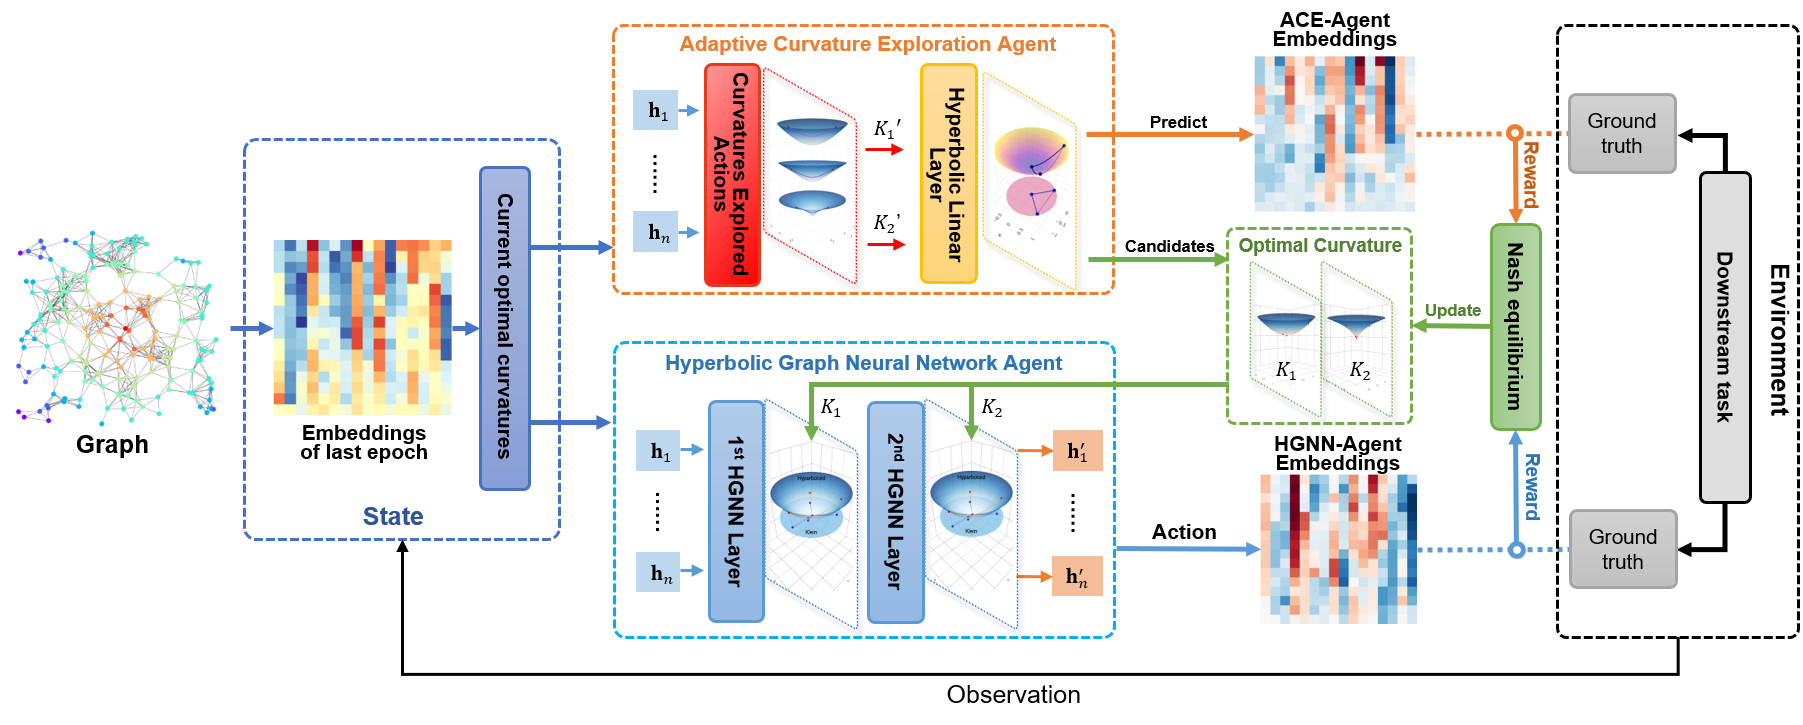
\includegraphics[width=0.9\textwidth]{figure/overall.png}
\caption{An illustration of RAHGNN architecture.}
\label{framework}
\end{figure*}

%Summary%
In summary, 
% with the curvature parameter $\zeta = \sqrt{ -K }$ and Equations~\eqref{graphdist},~\eqref{hyperdist2},  and~\eqref{hypergraphdist2}, 
we highlight two important conclusions as follows:
(1) Curvature determines the distance measure by adjusting for the distortion of space, which can measure representations capability with fusing the hierarchical structure and node features information in hyperbolic embedding space. 
(2) For hyperbolic geometric embedding, adjusting the curvature can better capture the hierarchy of the graph. 
However, an inappropriate curvature may degrade the representational capability of node features or semantics, especially in some classification tasks where node features are more important or using some "low tree-like" graphs. 

Based on these properties of curvature, we can solve the structural adaptive problem of hyperbolic graph representation learning as an optimal curvature selection problem of hyperbolic space. 
It provides a foundation for us to design an intuitive and effective solution. 